\documentclass[]{article}
\usepackage{lmodern}
\usepackage{amssymb,amsmath}
\usepackage{ifxetex,ifluatex}
\usepackage{fixltx2e} % provides \textsubscript
\ifnum 0\ifxetex 1\fi\ifluatex 1\fi=0 % if pdftex
  \usepackage[T1]{fontenc}
  \usepackage[utf8]{inputenc}
\else % if luatex or xelatex
  \ifxetex
    \usepackage{mathspec}
  \else
    \usepackage{fontspec}
  \fi
  \defaultfontfeatures{Ligatures=TeX,Scale=MatchLowercase}
\fi
% use upquote if available, for straight quotes in verbatim environments
\IfFileExists{upquote.sty}{\usepackage{upquote}}{}
% use microtype if available
\IfFileExists{microtype.sty}{%
\usepackage{microtype}
\UseMicrotypeSet[protrusion]{basicmath} % disable protrusion for tt fonts
}{}
\usepackage[margin=1in]{geometry}
\usepackage{hyperref}
\hypersetup{unicode=true,
            pdftitle={Final report},
            pdfauthor={Margot Chen, Qi Yang},
            pdfborder={0 0 0},
            breaklinks=true}
\urlstyle{same}  % don't use monospace font for urls
\usepackage{longtable,booktabs}
\usepackage{graphicx,grffile}
\makeatletter
\def\maxwidth{\ifdim\Gin@nat@width>\linewidth\linewidth\else\Gin@nat@width\fi}
\def\maxheight{\ifdim\Gin@nat@height>\textheight\textheight\else\Gin@nat@height\fi}
\makeatother
% Scale images if necessary, so that they will not overflow the page
% margins by default, and it is still possible to overwrite the defaults
% using explicit options in \includegraphics[width, height, ...]{}
\setkeys{Gin}{width=\maxwidth,height=\maxheight,keepaspectratio}
\IfFileExists{parskip.sty}{%
\usepackage{parskip}
}{% else
\setlength{\parindent}{0pt}
\setlength{\parskip}{6pt plus 2pt minus 1pt}
}
\setlength{\emergencystretch}{3em}  % prevent overfull lines
\providecommand{\tightlist}{%
  \setlength{\itemsep}{0pt}\setlength{\parskip}{0pt}}
\setcounter{secnumdepth}{0}
% Redefines (sub)paragraphs to behave more like sections
\ifx\paragraph\undefined\else
\let\oldparagraph\paragraph
\renewcommand{\paragraph}[1]{\oldparagraph{#1}\mbox{}}
\fi
\ifx\subparagraph\undefined\else
\let\oldsubparagraph\subparagraph
\renewcommand{\subparagraph}[1]{\oldsubparagraph{#1}\mbox{}}
\fi

%%% Use protect on footnotes to avoid problems with footnotes in titles
\let\rmarkdownfootnote\footnote%
\def\footnote{\protect\rmarkdownfootnote}

%%% Change title format to be more compact
\usepackage{titling}

% Create subtitle command for use in maketitle
\providecommand{\subtitle}[1]{
  \posttitle{
    \begin{center}\large#1\end{center}
    }
}

\setlength{\droptitle}{-2em}

  \title{Final report}
    \pretitle{\vspace{\droptitle}\centering\huge}
  \posttitle{\par}
    \author{Margot Chen, Qi Yang}
    \preauthor{\centering\large\emph}
  \postauthor{\par}
      \predate{\centering\large\emph}
  \postdate{\par}
    \date{2020/3/14}


\begin{document}
\maketitle

\hypertarget{beijing-pm2.5}{%
\section{Beijing PM2.5}\label{beijing-pm2.5}}

\hypertarget{introduction}{%
\subsection{Introduction}\label{introduction}}

Beijing, the capital city of China, has been fighting against
\texttt{PM2.5} pollution in recent years. \texttt{PM2.5} are fine
airborne particles less than 2.5μm that can cause severe damage to human
health by triggering lung cancer, heart diseases, stroke, and
respiratory infections. A Nature study pointed out that in 2016 only,
\texttt{PM2.5} was associated with over four million deaths worldwide.
In the past decades, the air quality in Beijing has been faced with
great pressure resulting from the rapid development of industry. In
order to secure its citizens' health, Chinese government has taken
action to mitigate the influence of \texttt{PM2.5} since September,
2013.\\
Previous studies showed that meteorological conditions(wind, humidity,
etc) could contribute to the formation of \texttt{PM2.5}. Therefore, we
speculate that there could be correlations between Beijing's
\texttt{PM2.5} concentration and the meteorological conditions in a
sufficient period of time.

\hypertarget{research-question}{%
\subsection{Research Question}\label{research-question}}

Our main research question is an \emph{exploratory} question: does the
\texttt{PM2.5} in Beijing correlates with meteorological conditions and
time? We speculate that there is indeed a correlation and that knowing
the meteorological conditions can support the assessment and even
prediction of air quality in Beijing. Sub-questions are as follows:\\
- \texttt{PM2.5} VS. physical parameters (dew point, temperature and
pressure).\\
- \texttt{PM2.5} VS. wind.\\
- \texttt{PM2.5} VS. special weather conditions (rain and snow).\\
- \texttt{PM2.5} VS. time (year, month, a time in a day).

\hypertarget{data-description}{%
\subsection{Data Description}\label{data-description}}

The
\href{https://archive.ics.uci.edu/ml/machine-learning-databases/00381/PRSA_data_2010.1.1-2014.12.31.csv}{dataset}
we used is from
\href{https://archive.ics.uci.edu/ml/datasets/Beijing+PM2.5+Data\#}{University
of California Irvine Machine learning Repository}. It was originally
uploaded by Songxi Chen in Peking University, China. This is an hourly
dataset containing the \texttt{PM2.5} concentration and meteorological
statistics in Beijing collected from Jan 1st, 2010 to Dec 31st, 2014.

Below are the variables in the dataset:

\begin{longtable}[]{@{}lll@{}}
\toprule
Variable & Type & Description\tabularnewline
\midrule
\endhead
year & Quantitative & Year of data in this row\tabularnewline
month & Quantitative & Month of data in this row\tabularnewline
day & Quantitative & Day of data in this row\tabularnewline
hour & Quantitative & Hour of data in this row\tabularnewline
\texttt{PM2.5} & Quantitative & \texttt{PM2.5} concentration
(ug/m\^{}3)\tabularnewline
DEWP & Quantitative & Dew Point (℃)\tabularnewline
TEMP & Quantitative & Temperature (℃)\tabularnewline
PRES & Quantitative & Pressure (hPa)\tabularnewline
cbwd & Categorical & Combined wind direction\tabularnewline
lws & Quantitative & Cumulated wind speed (m/s)\tabularnewline
ls & Quantitative & Cumulated hours of snow\tabularnewline
lr & Quantitative & Cumulated hours of rain\tabularnewline
\bottomrule
\end{longtable}

\hypertarget{exploratory-data-analysis-eda}{%
\subsection{Exploratory data analysis
(EDA)}\label{exploratory-data-analysis-eda}}

\hypertarget{correllogram}{%
\subsubsection{1.Correllogram}\label{correllogram}}

Our first step was to check if there are correlations between
meteorological conditions and \texttt{PM2.5} concentration using a
correllogram. The colors in the first row are very shallow and
corresponding values are close to zero, indicating weak correlations
between \texttt{PM2.5} concentration and meteorological conditions.

\begin{figure}
\centering
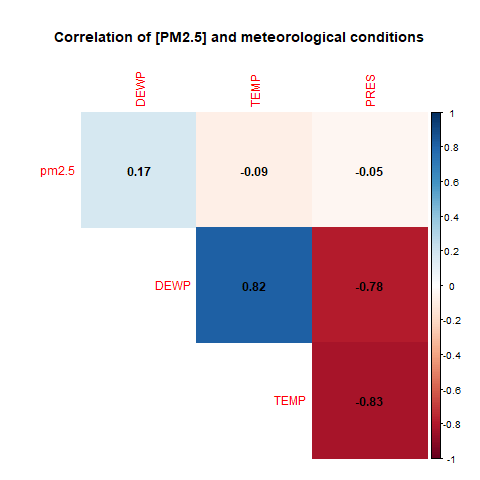
\includegraphics{../images/corr.png}
\caption{Figure 1.Correlation between PM2.5 concentration and dew point,
temperature or pressure}
\end{figure}

\hypertarget{faceted-histogram}{%
\subsubsection{2.Faceted histogram}\label{faceted-histogram}}

Next, we used a faceted histogram to check the distribution of
\texttt{PM2.5} under different wind directions. The Y axis in the image
below is the count of a certain PM2.5 concentration, indicating the
severity of PM2.5 pollution. Each facet stands for a wind direction*.\\
\emph{Only northeast, southwest, southeast and calm and variable were
recorded as the wind direction in the dataset; northwest was somehow
missed}

For different wind directions, the range of \texttt{PM2.5} concentration
is similar, but the absolute and relative frequency of a specific
\texttt{PM2.5} concentration are different: northwest and southeast tend
to have more recordings of low values.

\begin{figure}
\centering
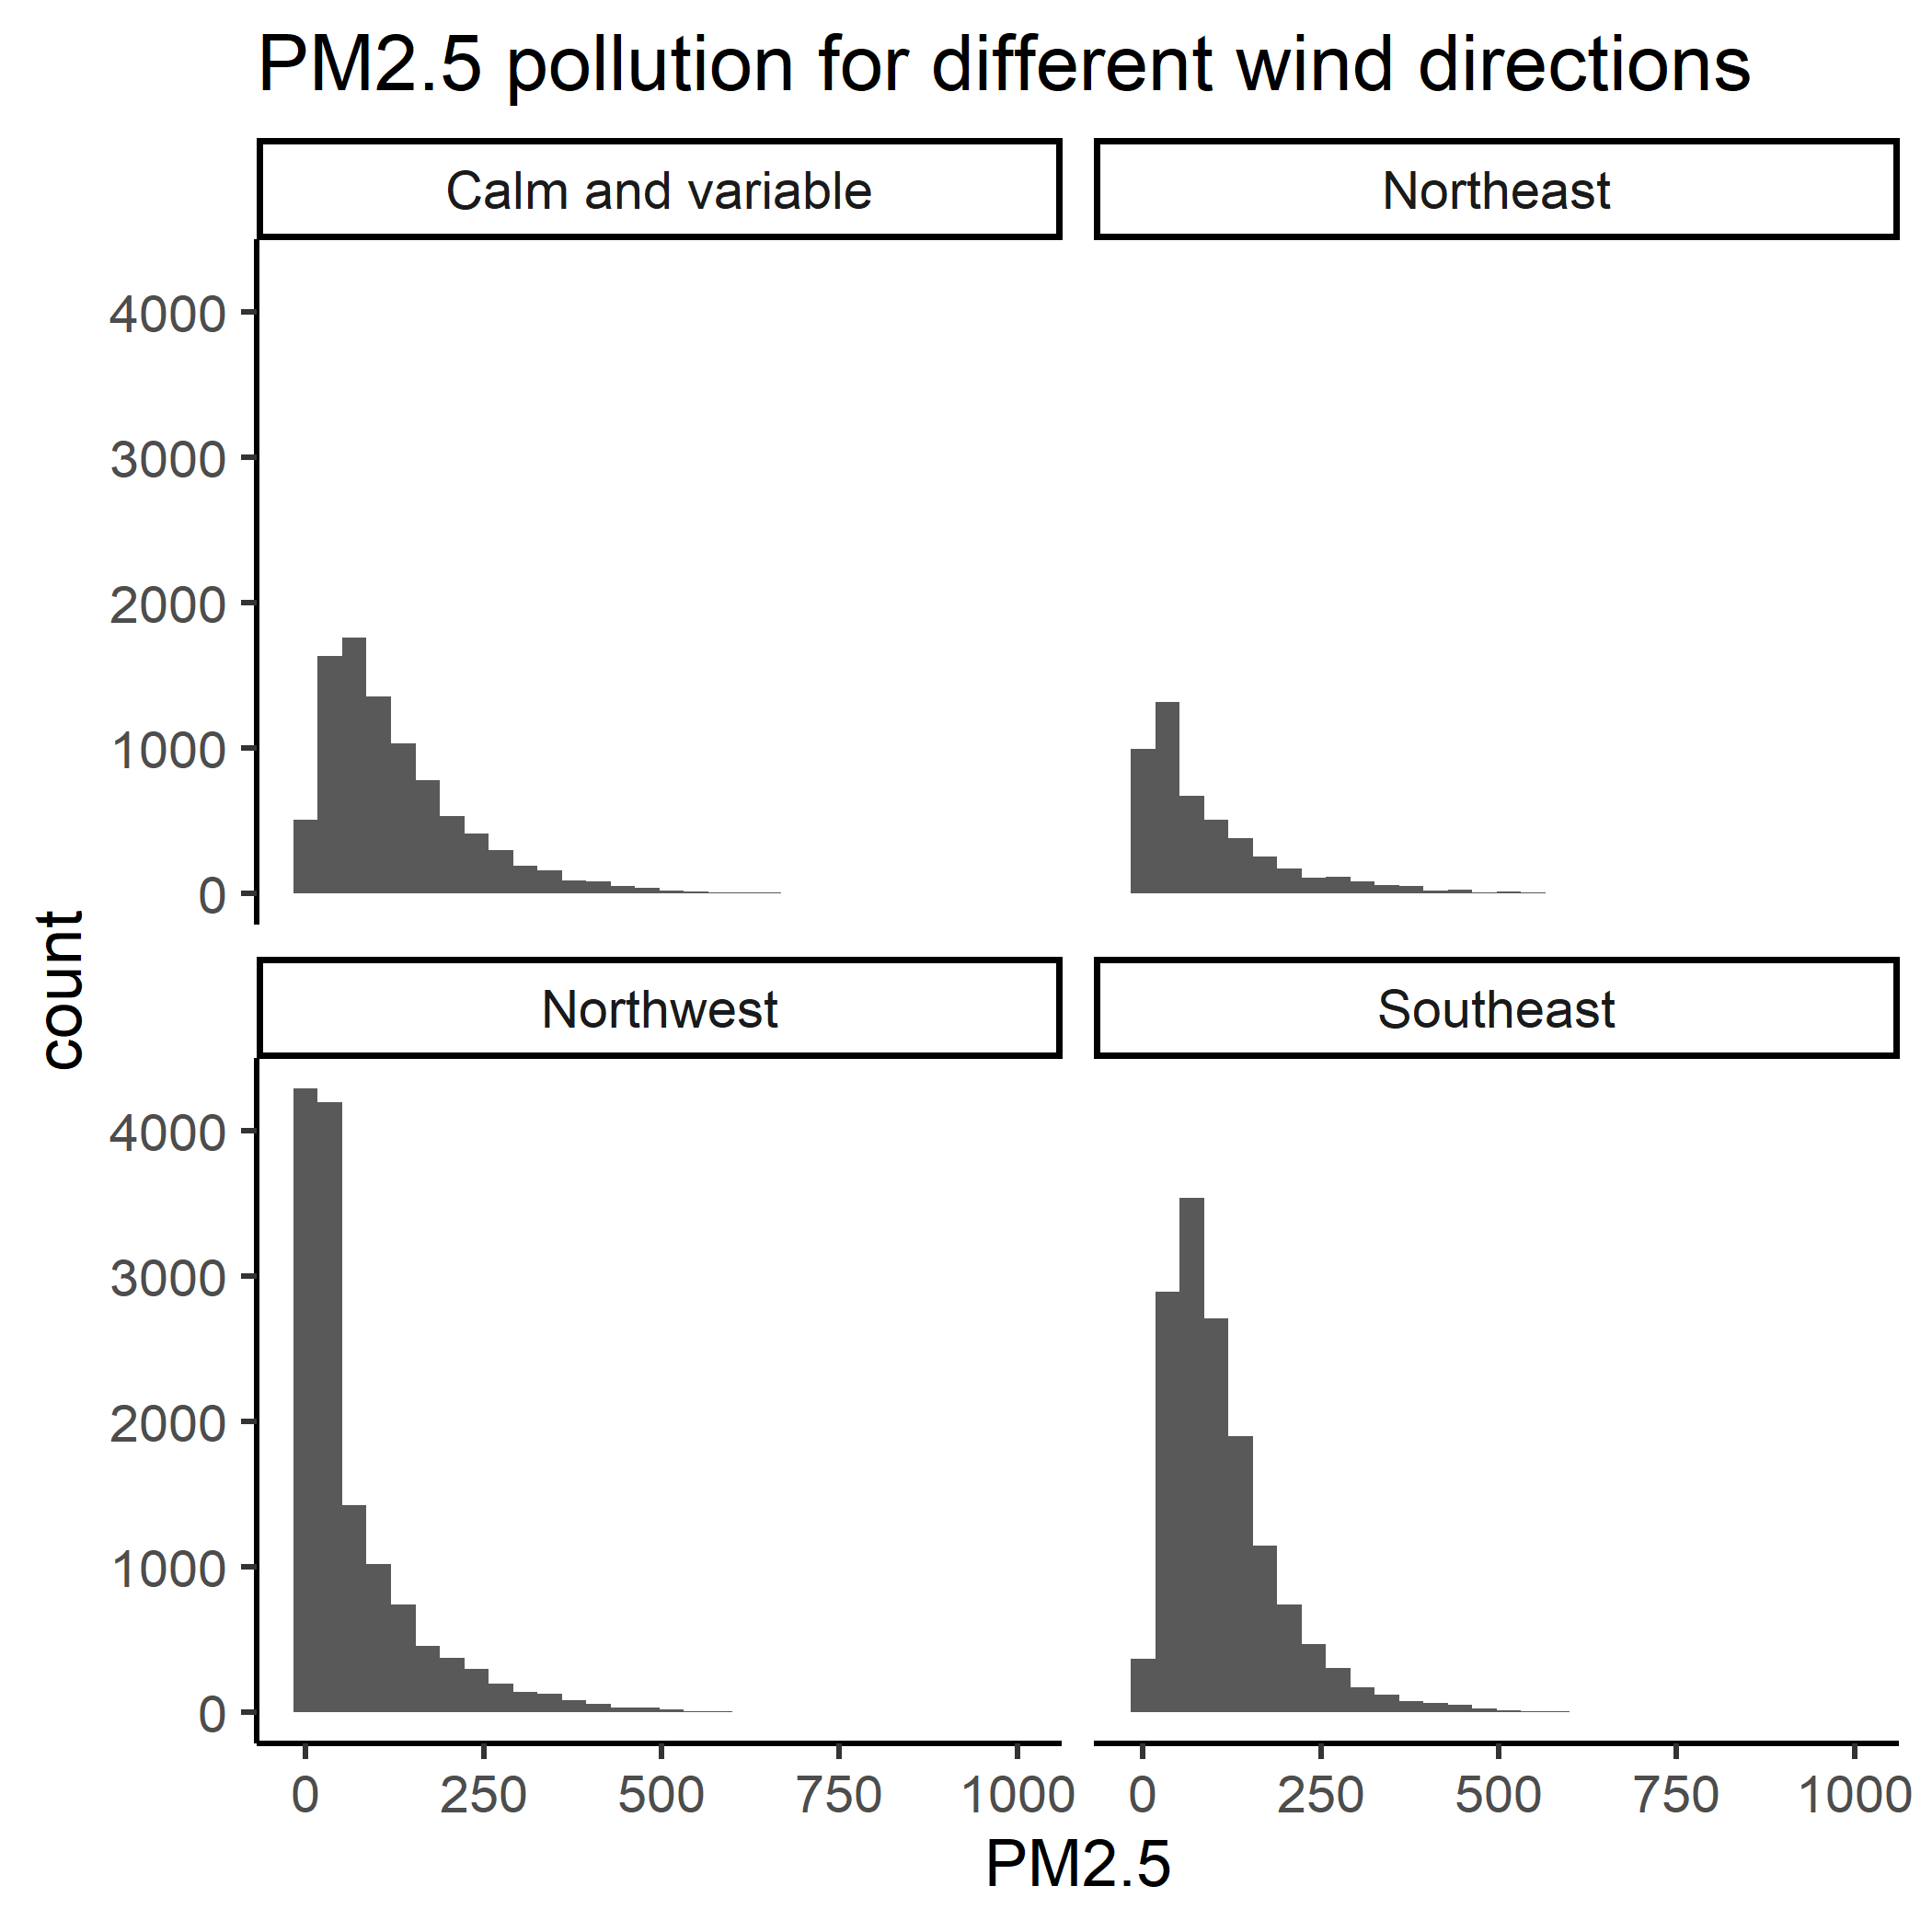
\includegraphics{../images/facted_hist.png}
\caption{Figure 2. PM2.5 pollution for different wind directions}
\end{figure}

\hypertarget{heat-map}{%
\subsubsection{3.Heat map}\label{heat-map}}

In addition to meteorological conditions, we are curious about the
correlation between \texttt{PM2.5} concentration and time, so we
generated a heat map. No significant color differences were found
between years (2013 and 2014) or within a day (morning, afternoon and
evening). However, the color varies in different months: October to
Februrary tend to have more dark colors compared to the other months.

\begin{figure}
\centering
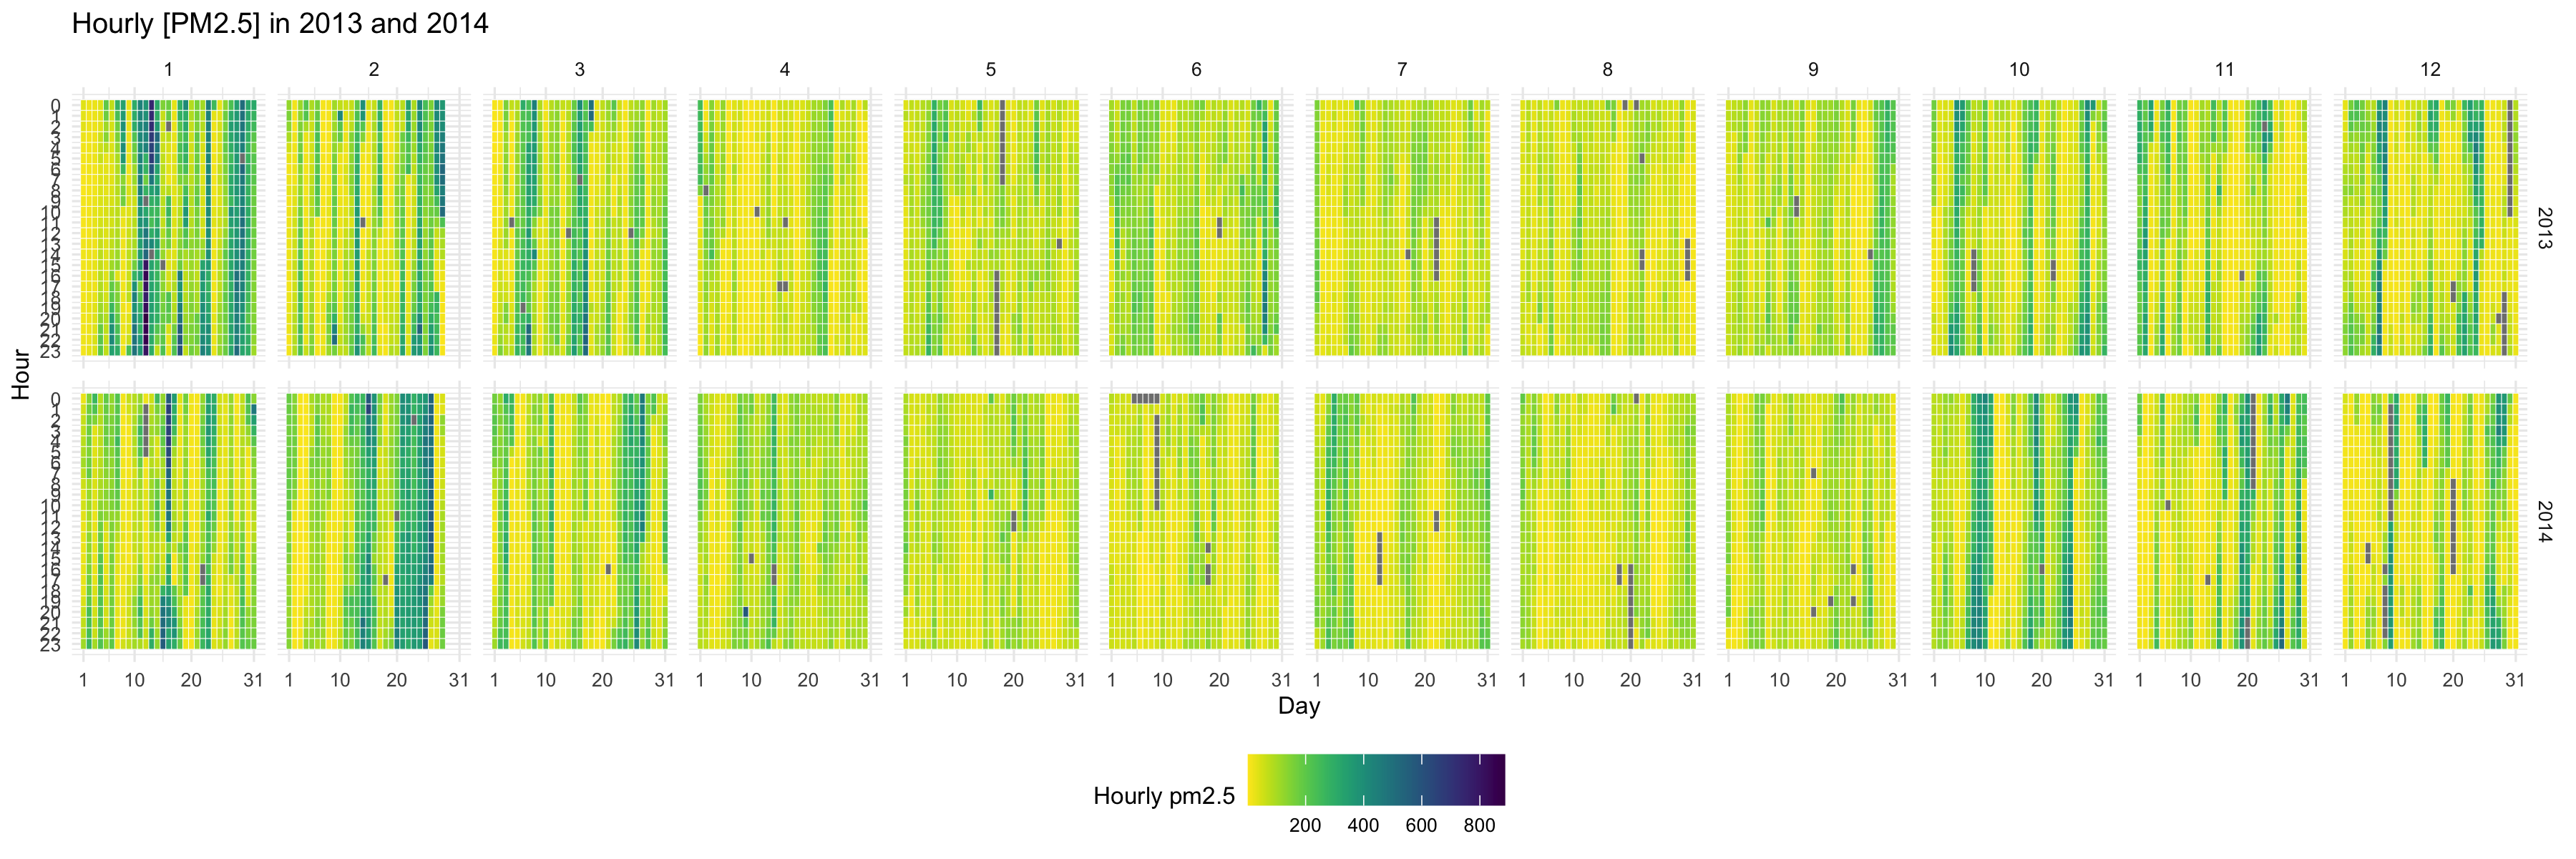
\includegraphics{../images/heatmap.png}
\caption{Figure 3. Hourly PM2.5 concentration in 2013 and 2014}
\end{figure}

Inspired by the heat map, we generated two more figures of
\texttt{PM2.5} concentration focusing on seasons and the trend across
years.

\hypertarget{histogram}{%
\subsubsection{4.Histogram}\label{histogram}}

The histogram emphasizes the severity of \texttt{PM2.5} pollution in
different seasons. We can see clearly that with the time going from
spring to winter, \texttt{PM2.5} concentration rises continously.

\begin{figure}
\centering
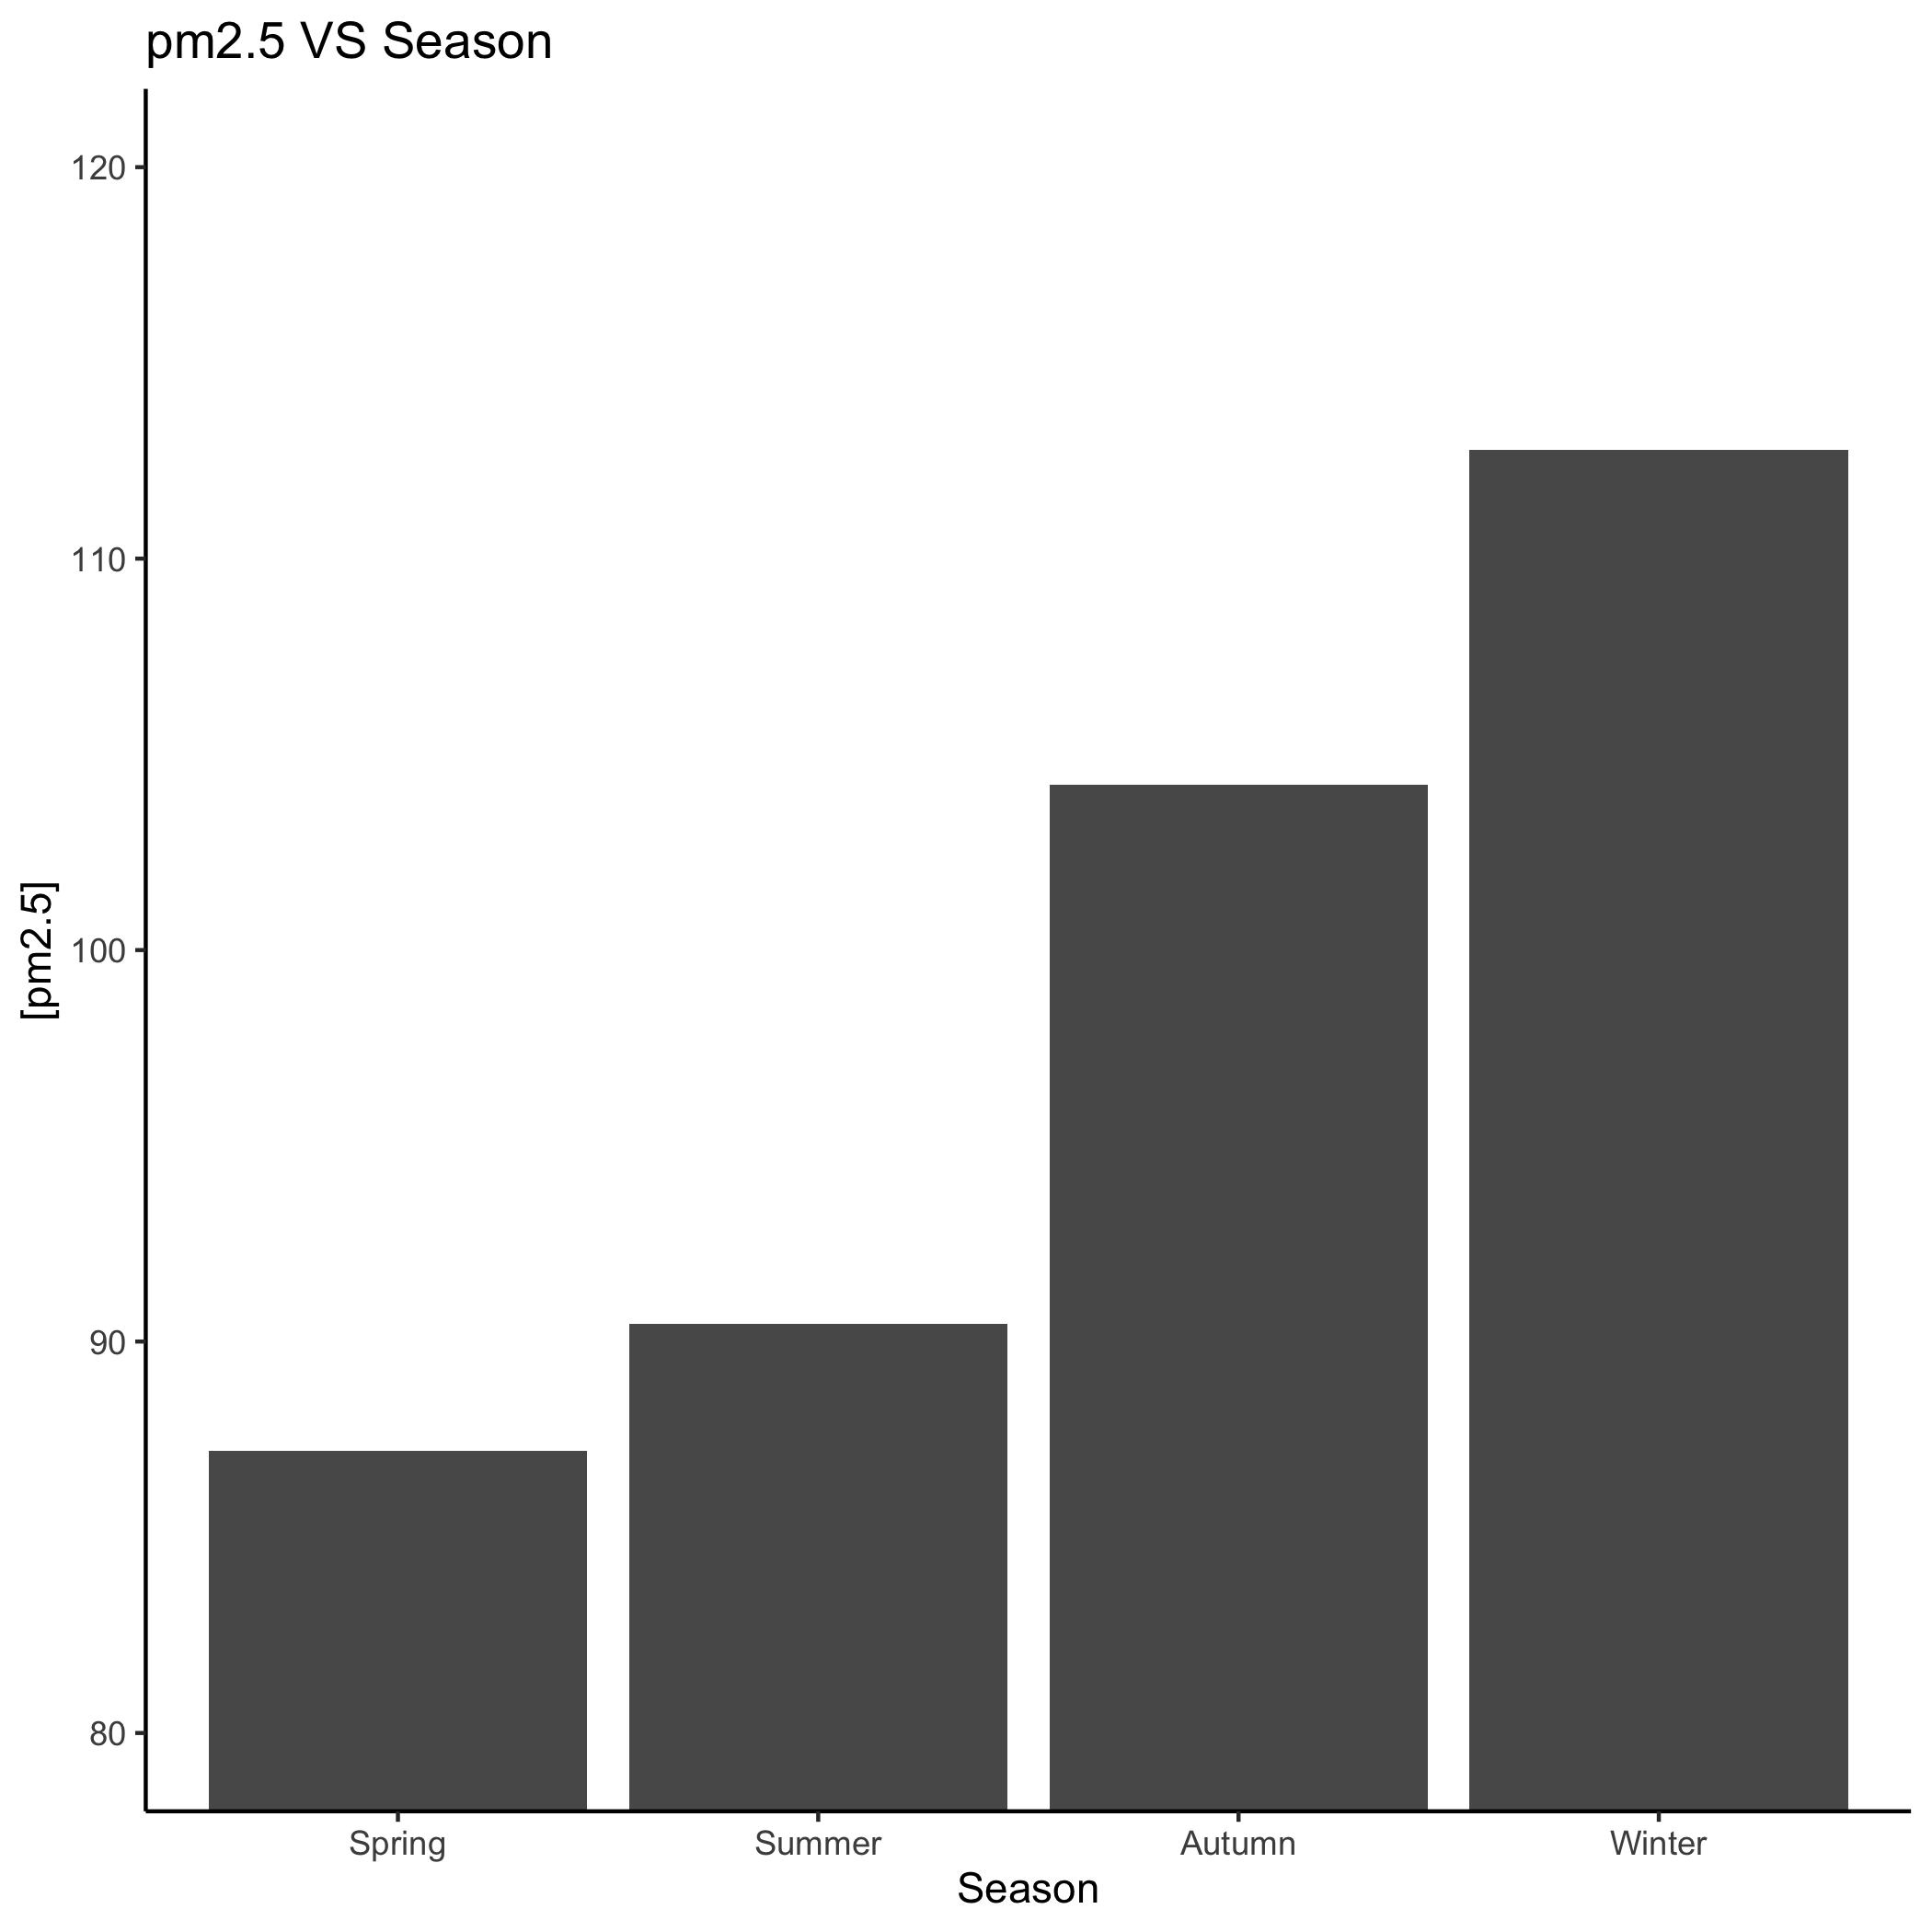
\includegraphics{../images/season_PM2.5.png}
\caption{Figure 4. PM2.5 pollution in different seasons}
\end{figure}

\hypertarget{line-chart}{%
\subsubsection{5.Line chart}\label{line-chart}}

The purpose of the line chart was to show the change of \texttt{PM2.5}
concentration across time. In general, the \texttt{PM2.5} concentration
seems to fluctuate, and peaks usually take place when new years come.
The blue dash line on the left of 2014 shows when the Chinese government
launched a plan to fight against the pollution, but it is hard to
observe a decrease in \texttt{PM2.5} concentration since this time.

\begin{figure}
\centering
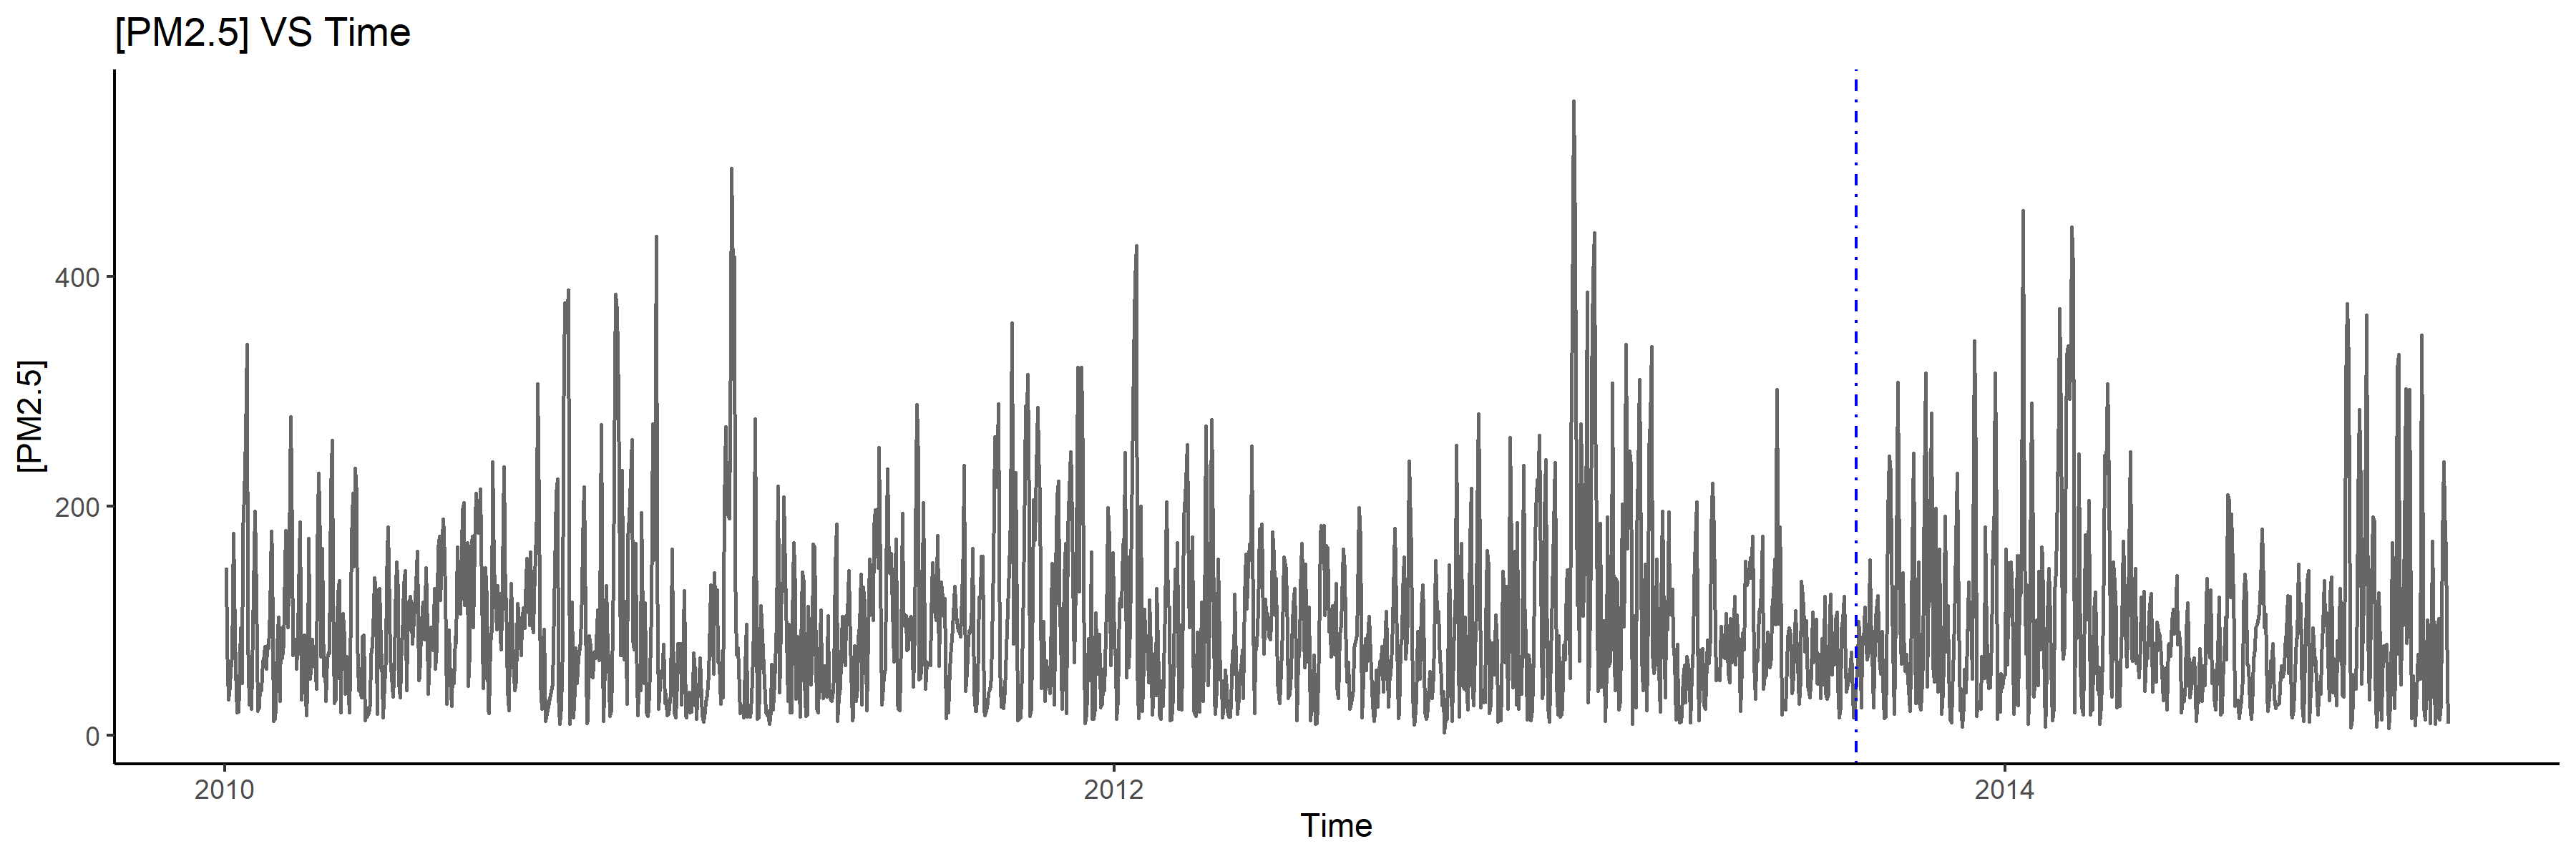
\includegraphics{../images/year_PM2.5.png}
\caption{Figure 5. PM2.5 concentration across years}
\end{figure}

\hypertarget{analysis-methods}{%
\subsection{Analysis methods}\label{analysis-methods}}

\hypertarget{results}{%
\subsection{Results}\label{results}}

In a nutshell, we find that \texttt{PM2.5} concentration is more likely
to change with time instead of meteorological conditons, which is rather
surprising as previous studies have shown correlation between
\texttt{PM2.5} and weather variables. Our first finding is that the
correlations between dew point (DEWP), temperature (TEMP) or pressure
(PRES) and \texttt{PM2.5}concentration are rather weak (Figure 1), so
the meteorological conditions can hardly predict the \texttt{PM2.5}
concentration.

In addition to the meteorological conditions studied above, wind is also
one of the important factors that can influence the formation of
\texttt{PM2.5}. According to Figure 2, \texttt{PM2.5} concentration
seems to have a similar range for all wind directions; and the pollution
is less serious when the wind comes from northwest and southeast.

\texttt{PM2.5} concentration changes within a year (Figure 3 and 4). The
pollution is more serious when it enters October and reaches its peak in
January/February. Besides, we didn't find significant differences across
years (Figure 3 and 5) or within a day.

\hypertarget{discussion}{%
\subsection{Discussion}\label{discussion}}

The weak correlations between \texttt{PM2.5} concentration and
meteorological conditions in Figure 1 are surprising to us as we
suspected that they should be strong. Based on
\href{https://www.atmos-chem-phys.net/18/5343/2018/acp-18-5343-2018.pdf}{previous
studies}, temperature and pressure are positively correlated with
\texttt{PM2.5} while humidity (dew points in this study) is negatively
correlated. This contradictory finding may result from the limitation of
\texttt{corrplot()}, and further analyses such as t-test are needed to
study the correlations.

Regardless of the wind direction, we found that \texttt{PM2.5}
concentration ranges from 0 to 994 and that during most of the time it
is below 72 (median). However, the severity of \texttt{PM2.5} pollution
differs across wind directions: when the wind comes from the northwest,
the severity seems to be the lowest, as lower PM2.5 concentrations are
more likely to occur. In comparison, winds coming from the northeast
tend to result in more serious pollution. We find this also surprising,
since the northernwest part of China are covered with more sand compared
to the northeast, which consists mostly of soil. This might because of
the number of recordings (absolute frequency) varies for different wind
directions, and more data is needed for further verification of this
result.

We attempted to see if there is any decrease in \texttt{PM2.5}
concentration that could possibly result from a plan of Chinese
government that aims to improve the air quality, which started in
September in 2013. However, we didn't find differences between 2013 and
2014, though there is a slight drop in the mean of\texttt{PM2.5}
concentration(before: 104.1933921; after: 97.4906558). The highest value
happened in 2013, which could possibly explain the government's
motivation to reduce the pollution, but it is hard to find an observable
decrease. This is reasonable since there could be lag for the action to
come into effect, and more data after 2014 is needed.

\texttt{PM2.5} pollution is more serious when it enters October and
reaches its peak in January/February. It is also worth noticing that the
increase between summer and autumn is the largest, suggesting that some
conditions changing at this time have greater contribution to the
formation of \texttt{PM2.5}, such as wind direction, temperature and dew
point, though the last two are not found to be correlated strongly with
\texttt{PM2.5} based on the correlogram. This finding is similar to
previous studies that point out that the worst case happens in autumn
and winter. It is reasonable when taking the conclusion drawn above
about the impact of the wind direction into account: located in the
northern part of China, Beijing experiences the wind coming from the
north from September to early March, which can result in a more serious
pollution. In comparison, the wind comes from the south from late March
to August, leading to less formation of \texttt{PM2.5} particles, so the
air condition is better.

By comparing different hours within a day, we were considering if
\texttt{PM2.5} concentration is higher in the morning and evening but
lower at noon. However, although our hypothesis can be true in some
winter days, \texttt{PM2.5} concentration seems to be stable within a
day during most of the time.

\hypertarget{references}{%
\subsubsection{References}\label{references}}

Liang, X., Zou, T., Guo, B., Li, S., Zhang, H., Zhang, S., Huang, H. and
Chen, S. X. (2015). Assessing Beijing's PM2.5 pollution: severity,
weather impact, APEC and winter heating. Proceedings of the Royal
Society A, 471, 20150257.


\end{document}
